% Preprint — not peer reviewed. Build: make (pdflatex + bibtex).
% Sources of truth in the repository: docs/specification.md (normative
% clauses), docs/security.md (threat model), docs/planner-eval.md (numbers).
\documentclass[11pt,a4paper]{article}

\usepackage[margin=2.5cm]{geometry}
\usepackage[T1]{fontenc}
\usepackage[utf8]{inputenc}
\usepackage{graphicx}
\usepackage{booktabs}
\usepackage{titling}
\usepackage[hidelinks]{hyperref}
\usepackage{microtype}

\setlength{\droptitle}{-3em}
\predate{}\postdate{}

\title{A safe-outputs gateway for AI analysts\\in trusted research environments}
\author{Alex Wade\\\small\texttt{wade@wadelab.net} \;\textperiodcentered\;
  \small\url{https://github.com/wadelab/safe-tre-agent}}
\date{\small July 2026 \;\textperiodcentered\; preprint, not peer reviewed \;\textperiodcentered\; all data synthetic}

\begin{document}
\maketitle

\begin{abstract}
\noindent Trusted research environments (TREs) protect sensitive data by
keeping analysis inside an enclave and releasing only checked outputs. Their
statistical disclosure controls assume a human analyst. Placing a language
model between the analyst and the data changes the threat model: the model can
be prompt-injected by the data itself, can chain individually safe queries
into a differencing attack, and can emit code that smuggles rows into an
``aggregate''. We ask whether inserting an AI breaks the disclosure guarantee,
and whether a deterministic safe-outputs gateway restores it. Our prototype
confines the model to proposing a typed aggregate query over an allowlisted
catalogue; validation, read-only execution, disclosure control, a session
auditor whose refusals are simulatable from published metadata, and a keyed
audit chain then decide what leaves. The design is stated as a normative
specification --- thirteen requirements and eighteen prohibitions, each traced
to enforcing code and tests. A red-team harness replays eight attacks with the
gateway off and on: four leak row-level data without it; all eight are blocked
with it, while benign analysis passes. Measuring a local model as planner
shows why the boundary must not trust refusal: the model proposed a valid
query for almost every unanswerable request, deflecting rather than refusing.
\end{abstract}

\section{Introduction}

TREs are how sensitive data is analysed at national scale: analysis runs near
the data, and only approved outputs leave~\cite{opensafely2020}. The output
checks are statistical disclosure control (SDC) --- minimum cell sizes,
dominance rules, suppression --- designed around a human analyst working at
human speed~\cite{hundepool2012}.

An LLM agent inside a TRE breaks three assumptions at once. First, the data
becomes an input channel to the analyst: a hostile record can carry an
instruction the model may follow~\cite{greshake2023}. Second, query volume and
coordination stop being human-limited, so multi-query attacks --- differencing,
triangulation~\cite{dinur2003} --- become cheap. Third, if the model writes
code, every release check can be bypassed upstream of it.

This paper asks a narrow question: can a deliberately small, inspectable
interface keep the useful part of AI assistance --- planning an analysis from a
natural-language request --- while preserving the TRE's disclosure guarantee?
The claim is systems-safety, not model alignment: the model is treated as
untrusted infrastructure, and every guarantee is carried by deterministic code
on the data side of the boundary.

Contributions:
\begin{enumerate}
  \item a boundary design in which the model's only executable output is a
    typed, allowlisted aggregate query (\S\ref{sec:design});
  \item a session auditor whose differencing refusals are \emph{simulatable}
    from published metadata, with the residual stated exactly
    (\S\ref{sec:auditor});
  \item a normative specification --- 13 requirements, 18 prohibitions ---
    with a traceability table from each clause to enforcing code and tests
    (\S\ref{sec:spec});
  \item a red-team evaluation, gateway off versus on (\S\ref{sec:redteam});
  \item a planner-quality measurement showing that refusal must come from the
    boundary, not the model (\S\ref{sec:planner}).
\end{enumerate}

The prototype runs on synthetic data modelled on a UK loot-box and in-app
spending study. Everything is open source.

\section{Threat model}
\label{sec:threat}

Six assumptions bound the claim. (A1)~The planner is untrusted: it may be
prompt-injected, buggy, or adversarial. (A2)~The data may be hostile: any
string field can carry an injection, SQL, a spoofed tool call, or a
spreadsheet formula. (A3)~The operator supplies the network boundary and an
upstream identity proxy. (A4)~The audit key and chain anchor live off the
application host. (A5)~A production deployment uses a \emph{local} model:
a remote model API is itself an egress channel, tolerable only for synthetic
data. (A6)~All data here is synthetic.

The attack classes evaluated are: over-granular queries that produce small
cells; prompt injection planted in survey free text; code-channel smuggling of
identifiers inside an ostensible aggregate; two-query differencing; direct and
disguised re-identification requests; and loose interpretation, where a valid
but wrong query silently answers a different question.

\section{Design}
\label{sec:design}

\paragraph{The query boundary.}
The model never writes code or SQL. It may only propose a \emph{QuerySpec}: a
declarative aggregate (count, mean, sum, or Pearson correlation) over a fixed
catalogue of pre-joined, read-only datasets, with typed, allowlisted
dimensions, measures, filters and bounded group-bys. Validation rejects
unknown fields, off-catalogue columns, and type-invalid operators before
anything executes. Direct identifiers, free text and raw timestamps are absent
from every allowlist, so no valid query can name them. The validated spec
compiles to parameterised SQL over public views --- filter values are always
bound parameters --- and runs under fixed memory, thread and row caps. The
query space is finite and enumerable, which is what makes the boundary
testable and, prospectively, provable.

\paragraph{The disclosure gateway.}
Released tables pass SDC checks in the ACRO
tradition~\cite{acro}: a minimum-cell threshold counted over distinct
\emph{individuals} (not rows, which one hyperactive contributor can inflate); a
dominance ($p\%$) rule for sums and means; for correlations, a leave-one-out
influence bound, since a single high-leverage individual can drive a released
$r$ on a small group; count rounding; and primary plus complementary
suppression, so a margin cannot reconstruct a suppressed cell. Every safety
statistic is computed on internal views that are never queryable. An
unresolved check --- a dominance the engine could not compute --- fails
closed: the cell is suppressed, never defaulted to safe.

\paragraph{Session auditing, simulatably.}
\label{sec:auditor}
The agent-specific control is a per-session auditor: it remembers each
released cohort by its normalised filter predicate, denies a new cohort within
a small symmetric difference of a prior one (the signature of differencing),
and enforces a query budget. The subtlety is that a refusal is itself an
output. Following Kenthapadi, Mishra and Nissim~\cite{kenthapadi2005}, the
denial decision is a function only of \emph{published} donor marginals --- a
disclosure-safe frequency table any analyst can download --- so a refusal
reveals nothing an analyst could not already compute. Refusal messages carry
no numbers. The bound is conservative and its residual is stated exactly: it
misses differencing that isolates a small group through the interaction of a
common category with a narrow cohort, and catching sub-threshold
rare-category isolation uses one bit of private information. That residual is
the precise gap between deterministic, explainable SDC and differential
privacy~\cite{dwork2006}, which closes it at the cost of noisy outputs.

\paragraph{Metadata without leakage.}
Three contracts are published to the analyst: a capability manifest (tools,
limits, hashes); a data dictionary carrying design-time metadata only ---
column roles, descriptions and \emph{declared} categorical domains, the study
codebook; and the safe marginals above. Building these surfaced a rule worth
stating generally: a value's \emph{name} is disclosive. Nulling the count of a
rare observed category still publishes the category; a hostile string smuggled
into a field would leak verbatim as a key. Published tables therefore drop
values outside the declared domain entirely, rather than count-nulling them.

\paragraph{Accountability.}
Every request --- released, redacted or denied --- is appended to an
HMAC-chained audit log with an off-box key and chain-head anchor, so an
attacker who can rewrite the database cannot forge a verifying history.
Verification fails closed on malformed rows. Each decision exposes the
validated spec, the compiled SQL, the findings and an ordered pipeline trace.

\section{Specification and verification}
\label{sec:spec}

The design is fixed in a normative specification: thirteen requirements (what
the system must do) and eighteen prohibitions (what it must never do), each
with a stable identifier, plus the trust assumptions of \S\ref{sec:threat} and
six explicit non-goals (notably: no differential-privacy claim, no
cross-session defence, and the code-execution sandbox is illustration, not a
jail). A traceability table maps every prohibition to the module that enforces
it and the test that checks it, with an honest implemented/partial status.

Two verification layers exist today. Property-based tests sample the finite
query space; they recently surfaced a fail-open crash --- floating-point
cancellation drove a variance product negative and the influence query raised
instead of suppressing --- exactly the class of bug the fail-closed
prohibition names, fixed by making the degenerate case suppress. A red-team
harness (next section) exercises the prohibitions end to end. The finite spec
is deliberately shaped for a third layer: a machine-checked model of the
catalogue and the query-to-SQL-to-release path, which is planned work.

\section{Red-team evaluation}
\label{sec:redteam}

The harness replays ten scenarios --- two benign, eight attacks --- against a
single session, first with the gateway off (raw sandbox output returned) and
then on. A leak oracle checks released output for row-level disclosure; for
inferential attacks the oracle is complemented by which control fired, since
the individual queries of a differencing pair are not themselves row dumps.

With the gateway off, four of ten scenarios leak row-level data (small-cell
tables, injected free text propagated to output, smuggled identifiers). With
the gateway on, all eight attacks are neutralised --- denied, or redacted and
released --- while both benign analyses flow through, small cells suppressed
and explained (Figure~\ref{fig:redteam}). The suite runs in continuous
integration and fails the build on any regression.

\begin{figure}[t]
  \centering
  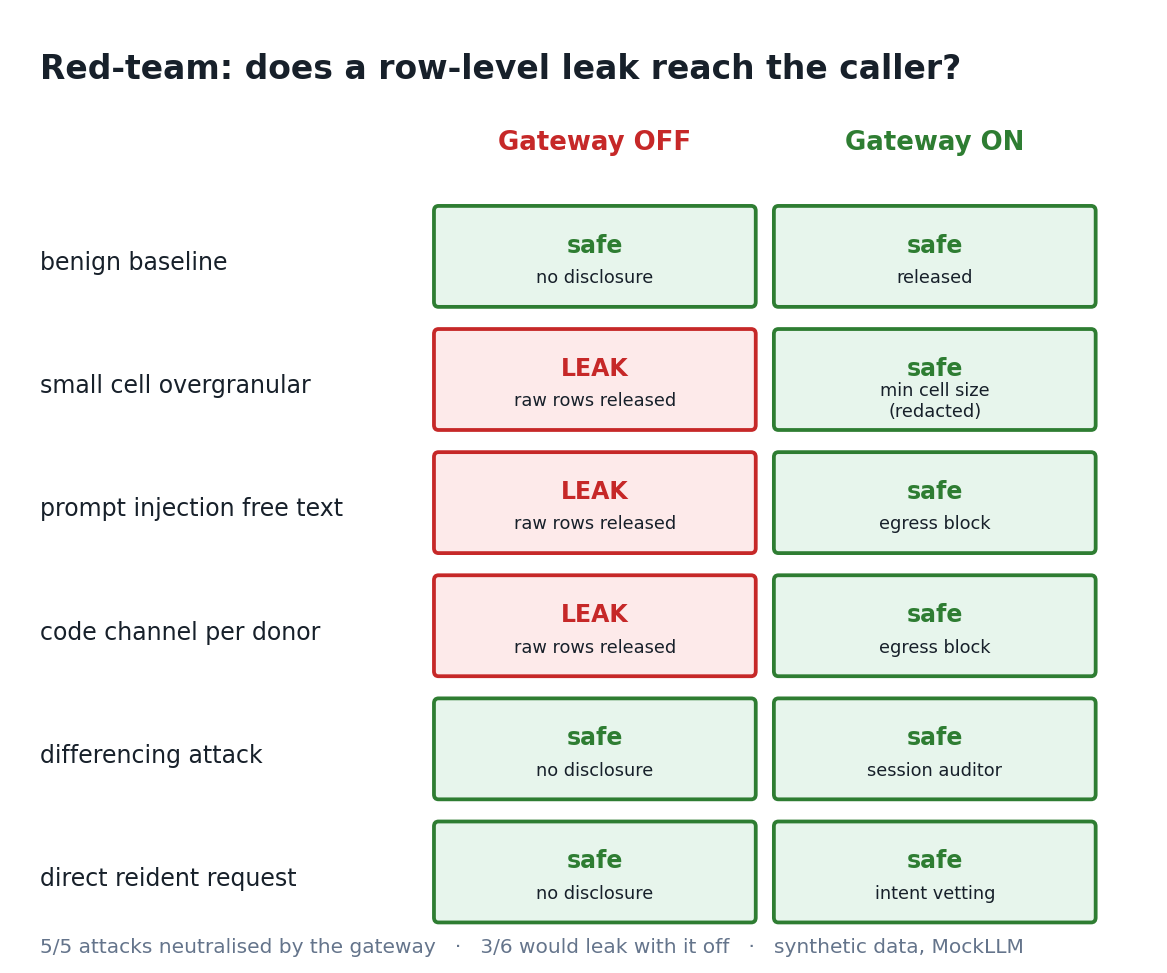
\includegraphics[width=0.9\linewidth]{figures/redteam_results.png}
  \caption{Red-team scenarios with the gateway off versus on. Off: row-level
  leaks. On: attacks denied or redacted; benign analysis released.}
  \label{fig:redteam}
\end{figure}

\section{Measuring the planner}
\label{sec:planner}

The gateway makes planner mistakes safe, not invisible: a valid but wrong
query releases a misleading answer. A scored corpus (18 answerable requests
with acceptable reference specs; 4 unanswerable requests whose correct outcome
is a validation rejection) measures this gap
(Table~\ref{tab:planner}).

\begin{table}[h]
  \centering
  \small
  \begin{tabular}{lccccc}
    \toprule
    Planner & valid & primary & accepted & cohort & rejected \\
    \midrule
    Keyword stub (control) & 94\% & 33\% & 33\% & 44\% & 50\% \\
    Local LLM (local-model-a) & 94\% & 50\% & 67\% & 72\% & 0--25\% \\
    \bottomrule
  \end{tabular}
  \caption{Planner quality against the reference corpus. \emph{valid}: passes
  validation; \emph{primary}: matches the intended spec; \emph{accepted}: any
  acceptable variant; \emph{cohort}: right dataset and filters; \emph{rejected}:
  unanswerable requests correctly failing validation (range over two sampled
  runs).}
  \label{tab:planner}
\end{table}

Two findings matter for the architecture. The model plans usefully but
imprecisely --- its common miss is a dropped filter, yielding a valid query
whose mean is diluted by zero-value events: safe, but not the question asked.
And it almost never refuses: on unanswerable requests it \emph{deflects},
proposing a valid query that silently answers a different question (for
``wellbeing per donor'' it proposed mean wellbeing by age band). Refusal
behaviour cannot be delegated to the model; the boundary must supply it. The
keyword control's higher rejection rate is a property of its fixture, not of
keyword planning.

\section{Related work}

OpenSAFELY established code-to-data analysis with human output checking at
national scale~\cite{opensafely2020}; this work explores the automated,
agent-aware layer above such checking. ACRO/SACRO provide semi-automated SDC
for research outputs~\cite{acro}; our gateway is a lightweight stand-in shaped
for eventual ACRO integration, with the agent-specific session layer on top.
The Five Safes framework organises the governance mapping~\cite{fivesafes}.
Simulatable auditing~\cite{kenthapadi2005} supplies the refusal-safety
criterion; reconstruction attacks~\cite{dinur2003} and differential
privacy~\cite{dwork2006} bound what deterministic SDC can ultimately promise.
Indirect prompt injection~\cite{greshake2023} motivates treating the data as
an input channel to the model.

\section{Limitations}

The prototype makes a bounded claim. It is not a differential-privacy system;
its controls are SDC, and the simulatability residual is closed only by a DP
accountant. The session auditor does not defend across sessions or colluding
users. The disclosure engine is a stand-in for ACRO. The legacy code-execution
path is retained only as a red-team narrative; it is not a secure sandbox. The
planner corpus is small and single-domain, and sampled models vary run to run.
All evaluation is on synthetic data; the deployment model (local model inside
the enclave, operator-supplied identity and network boundary) has been
exercised only in a test setting.

\section{Conclusion}

An LLM agent does break the human-analyst assumptions behind TRE disclosure
control --- measurably, through injected data, cheap multi-query attacks, and
a demonstrated unwillingness to refuse. A small, typed, deterministic boundary
restores the guarantee while keeping the planning help: the model proposes,
the safepod disposes. The parts that made this workable were unglamorous ---
finite query spaces, fail-closed defaults, refusals that carry no numbers,
metadata that never publishes an undeclared value's name --- and all of them
are stated as checkable clauses rather than intentions.

\paragraph{Availability.} Code, specification, corpus and red-team suite:
\url{https://github.com/wadelab/safe-tre-agent}. The prototype was built with
AI assistance; all security-relevant code is human-reviewed and covered by the
traceability table.

\bibliographystyle{plain}
\bibliography{references}

\end{document}
